In this project, we are the mixture of waterfall and agile process development model shown in the Figure 2. 
\paragraph{} Waterfall model can produce rigorous documentation and a reliable governance with the phased approach, which can help facilitating production of complete documentation and software design, such as gathering user requirement, freeze requirements, begin coding, move to testing, etc. The initial phase of the project is focused on gathering the software requirement.There will be two official milestones and several internal project team milestones, in order to deliver the product on time. Project deliverables are divided into sub-activities and for each activity a development cycle will be followed which will include different phases such as design, development, testing..

\paragraph{} Agile process development model (Shown on Fig.2) provides high customer satisfaction due to continuous delivery of the software modules and ensures the high quality software development. This model has advantages such as no planning is required to start the project as compared to other traditional software development models such as water fall in which project team makes strict promises to the client by doing requirement analysis and planning. This model is very easy to manage and provides great flexibility to the project team and client.

\begin{figure}
	\centering
	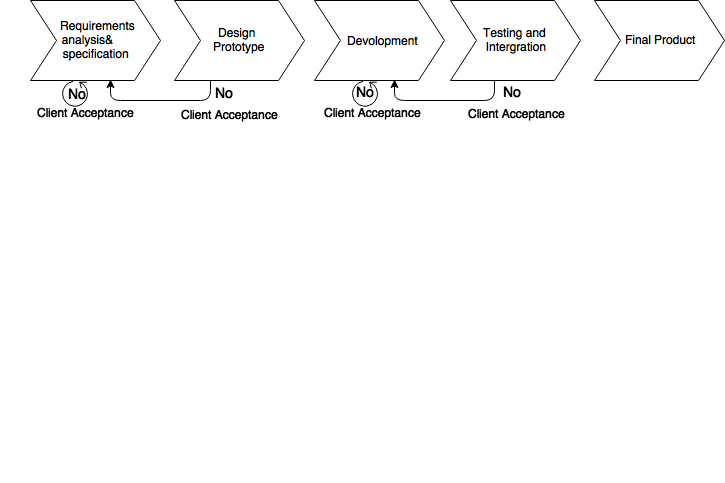
\includegraphics[width=0.9\textwidth]{model.png}
	\caption{\label{fig:process_model}The mixture  model diagram}
\end{figure}


